\documentclass[11pt]{article}
\usepackage{amssymb,amsmath}
\usepackage{graphicx} 

\title{Splotch on GPUs using the CUDA Paradigm}
%\author{M. Rivi, C. Gheller, M.Krokos}
\author{.........}

\begin{document}
\maketitle

\section{Introduction}
\label{sec:intro}

blah blah blah

\section{Splotch Overview}
\label{sec:overview}

The software package is completely self-contained with no dependencies from external libraries (apart of course from those needed for parallelism and to support specific file formats, e.g. HDF5 \cite{hdf5} ). The code is pure C++ and compilation is straightforward through suitable makefile scripts. The operational scenario involves a number of distinct stages as below: 

\begin{itemize}
\item
{\it Data Loading} - Several readers are available supporting different formats. As a minimum ($x$, $y$, $z$) scalars are required representing the positions of particles in cartesian or any other (user-defined) customised coordinate systems.
\item
{\it Rasterization and Processing} - Firstly, normalisation together with other necessary 
calculations (e.g. logarithms of processed quantities) are performed. Secondly, particle 
coordinates and other geometric quantities (e.g. smoothing lengths - see below) are 
\item
{\it Rendering} - The contributions of individual particles to pixels of the final 
image are calculated solving the radiative transfer equation  \cite{1991par..book.....S}:
\begin{equation}\label{rad}
\frac{d\bf{I_{\lambda}}(x)}{dx}=(\bf{E}_p-\bf{A}_p\bf{I_{\lambda}}(x))\rho_p^{\lambda}(x),
\end{equation}
where $I_{\lambda}$ is the intensity of pixel $x$ for the three color components, 
$\lambda$ = R, G and B, $\rho_p^{\lambda}(x)$ is a quantity transported by the particle $p$ 
(e.g. temperature or density),

Equation \eqref{rad} is solved for each color component using a finite differences 
approximation along the lines of sight originating from each pixel. Each 
particle contributes to a pixel according to a Gaussian distribution:
\begin{equation}\label{smooth}
\rho_p^{\lambda}(x)=\rho_p^{\lambda}\exp(-r^2/\sigma_p^2),
\end{equation}
where $\rho_p^{\lambda}$ is the value read from the data file, 
$r$ is the distance of the particle $p$ from the pixel and 
$\sigma_p$ is a smoothing length deployed for modelling the particle size. 
Although individual particles contribute to all pixels of the rendered images, 
for practical purposes it is handy to use a compact support of this
Gaussian distribution. The distribution is considered to be zero at a given
distance $\chi\cdot\sigma_p$, where $\chi$ is a suitably-defined multiplicative factor.
Any rays passing $p$ at larger distances are unaffected by $\rho_p$.

\section{The GPU Code}
\label{sec:gpu-code}

\subsection{The CUDA programming model} 
\label{sec:cuda}

\begin{figure}
\centering
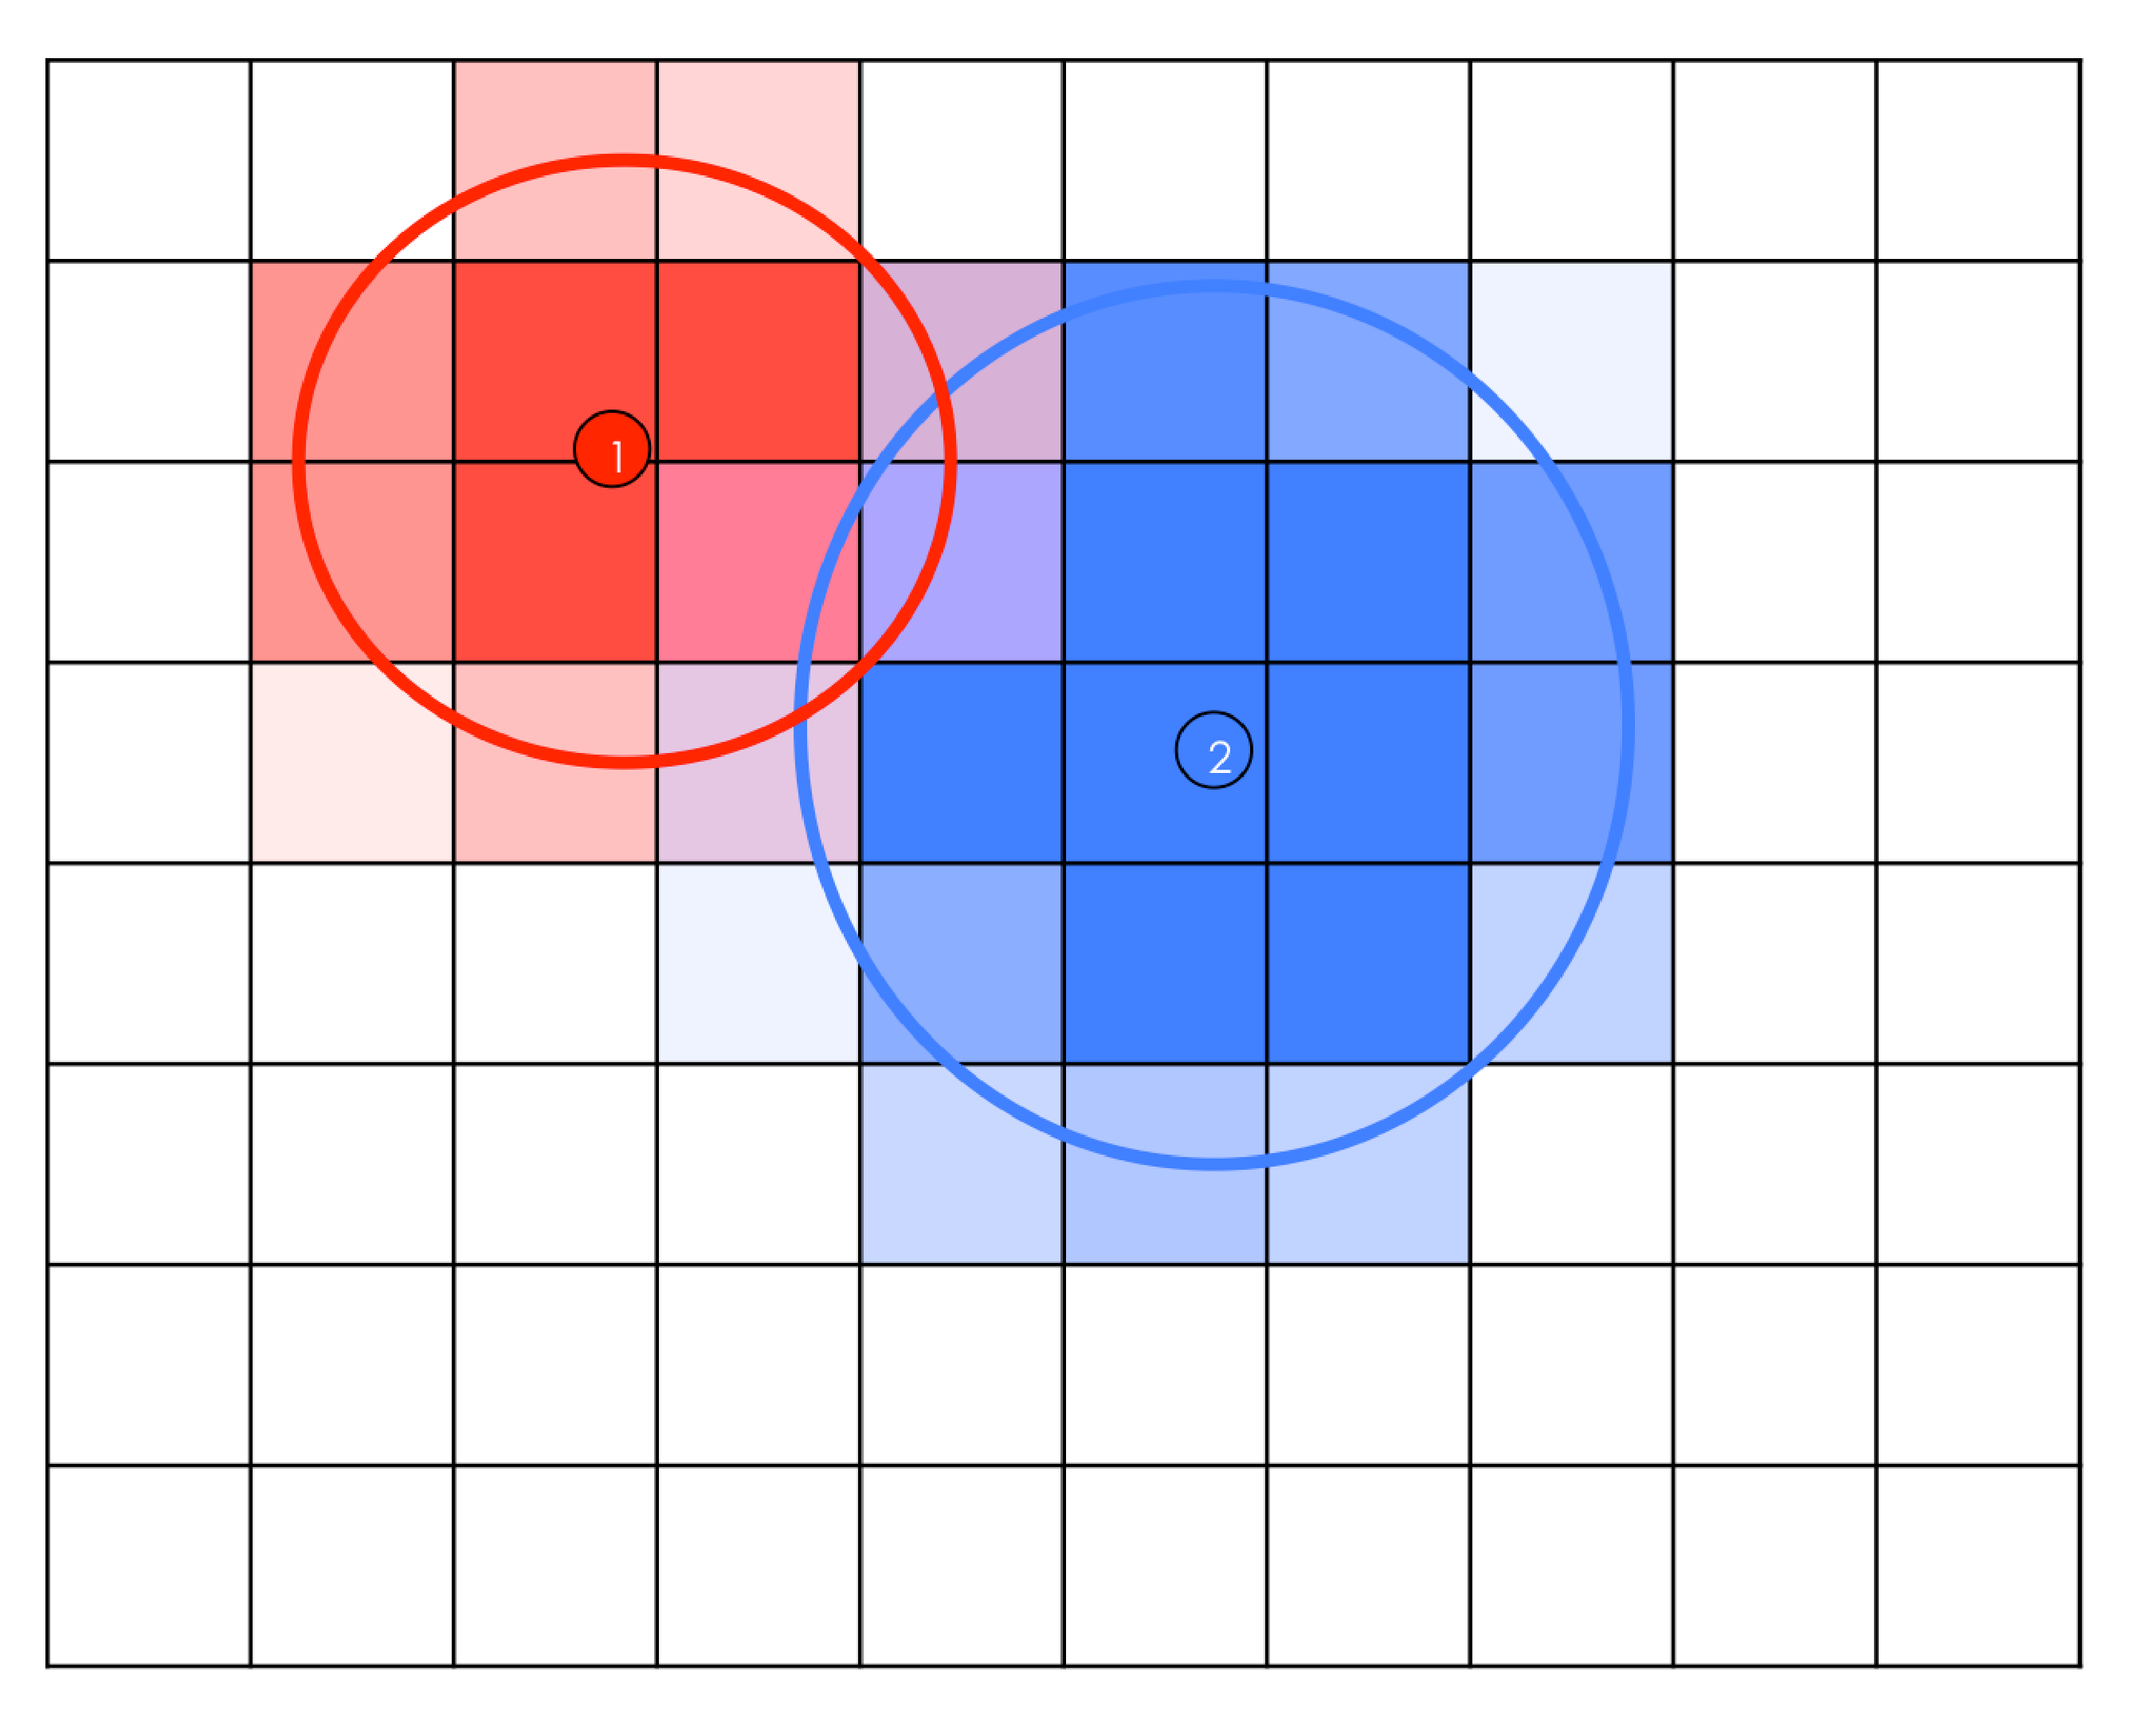
\includegraphics[scale=0.2]{images/particles.eps}
\caption{Two particles with different radii influencing the same pixels.}
\label{fig:particles}
\end{figure}

Equation \eqref{tmgpu} shows that the performance related to global-shared memory 
data transfers
depends on the two parameters $N_{load,p}$ and $N_{store,p}$, that quantify the
total amount of data transferred from the global to the shared memories 
and back, whose performance depends on the memory bandwidth.

The $T_{Mgpu}$ term depends linearly on the image size. Once more, 
for large datasets, this term appears to be negligible. However, since
particles falling outside the field of view are not processed (``inactive'' particles,
see Figure~\ref{fig:fov} for an example),
depending on the camera position, the ratio between the number of active particles
and the number of pixels can substantially decrease. Therefore, 
the image related term can give a meaningful contribution to
the computing time. 

A critical term of equation \eqref{tmgpu} is represented by the memory access
latency $N_{Ngpu} \nu_{mem}$. The access to memory is slow in comparison to
the available bandwidth, so a small number of accesses, $N_{Ngpu}$, is crucial
to the performance. This can be achieved by standard caching strategies, that
however are effective only if data coalesced access (in particular data contiguity) is guaranteed. In other words,

For the Rendering stage, a simple {\it one-thread-per-particle} approach
cannot be adopted (see Section~\ref{sec:model}). Furthermore, memory usage must be carefully managed.

\subsection{Rendering algorithm design}
\label{sec:design}

\begin{figure}
\centering
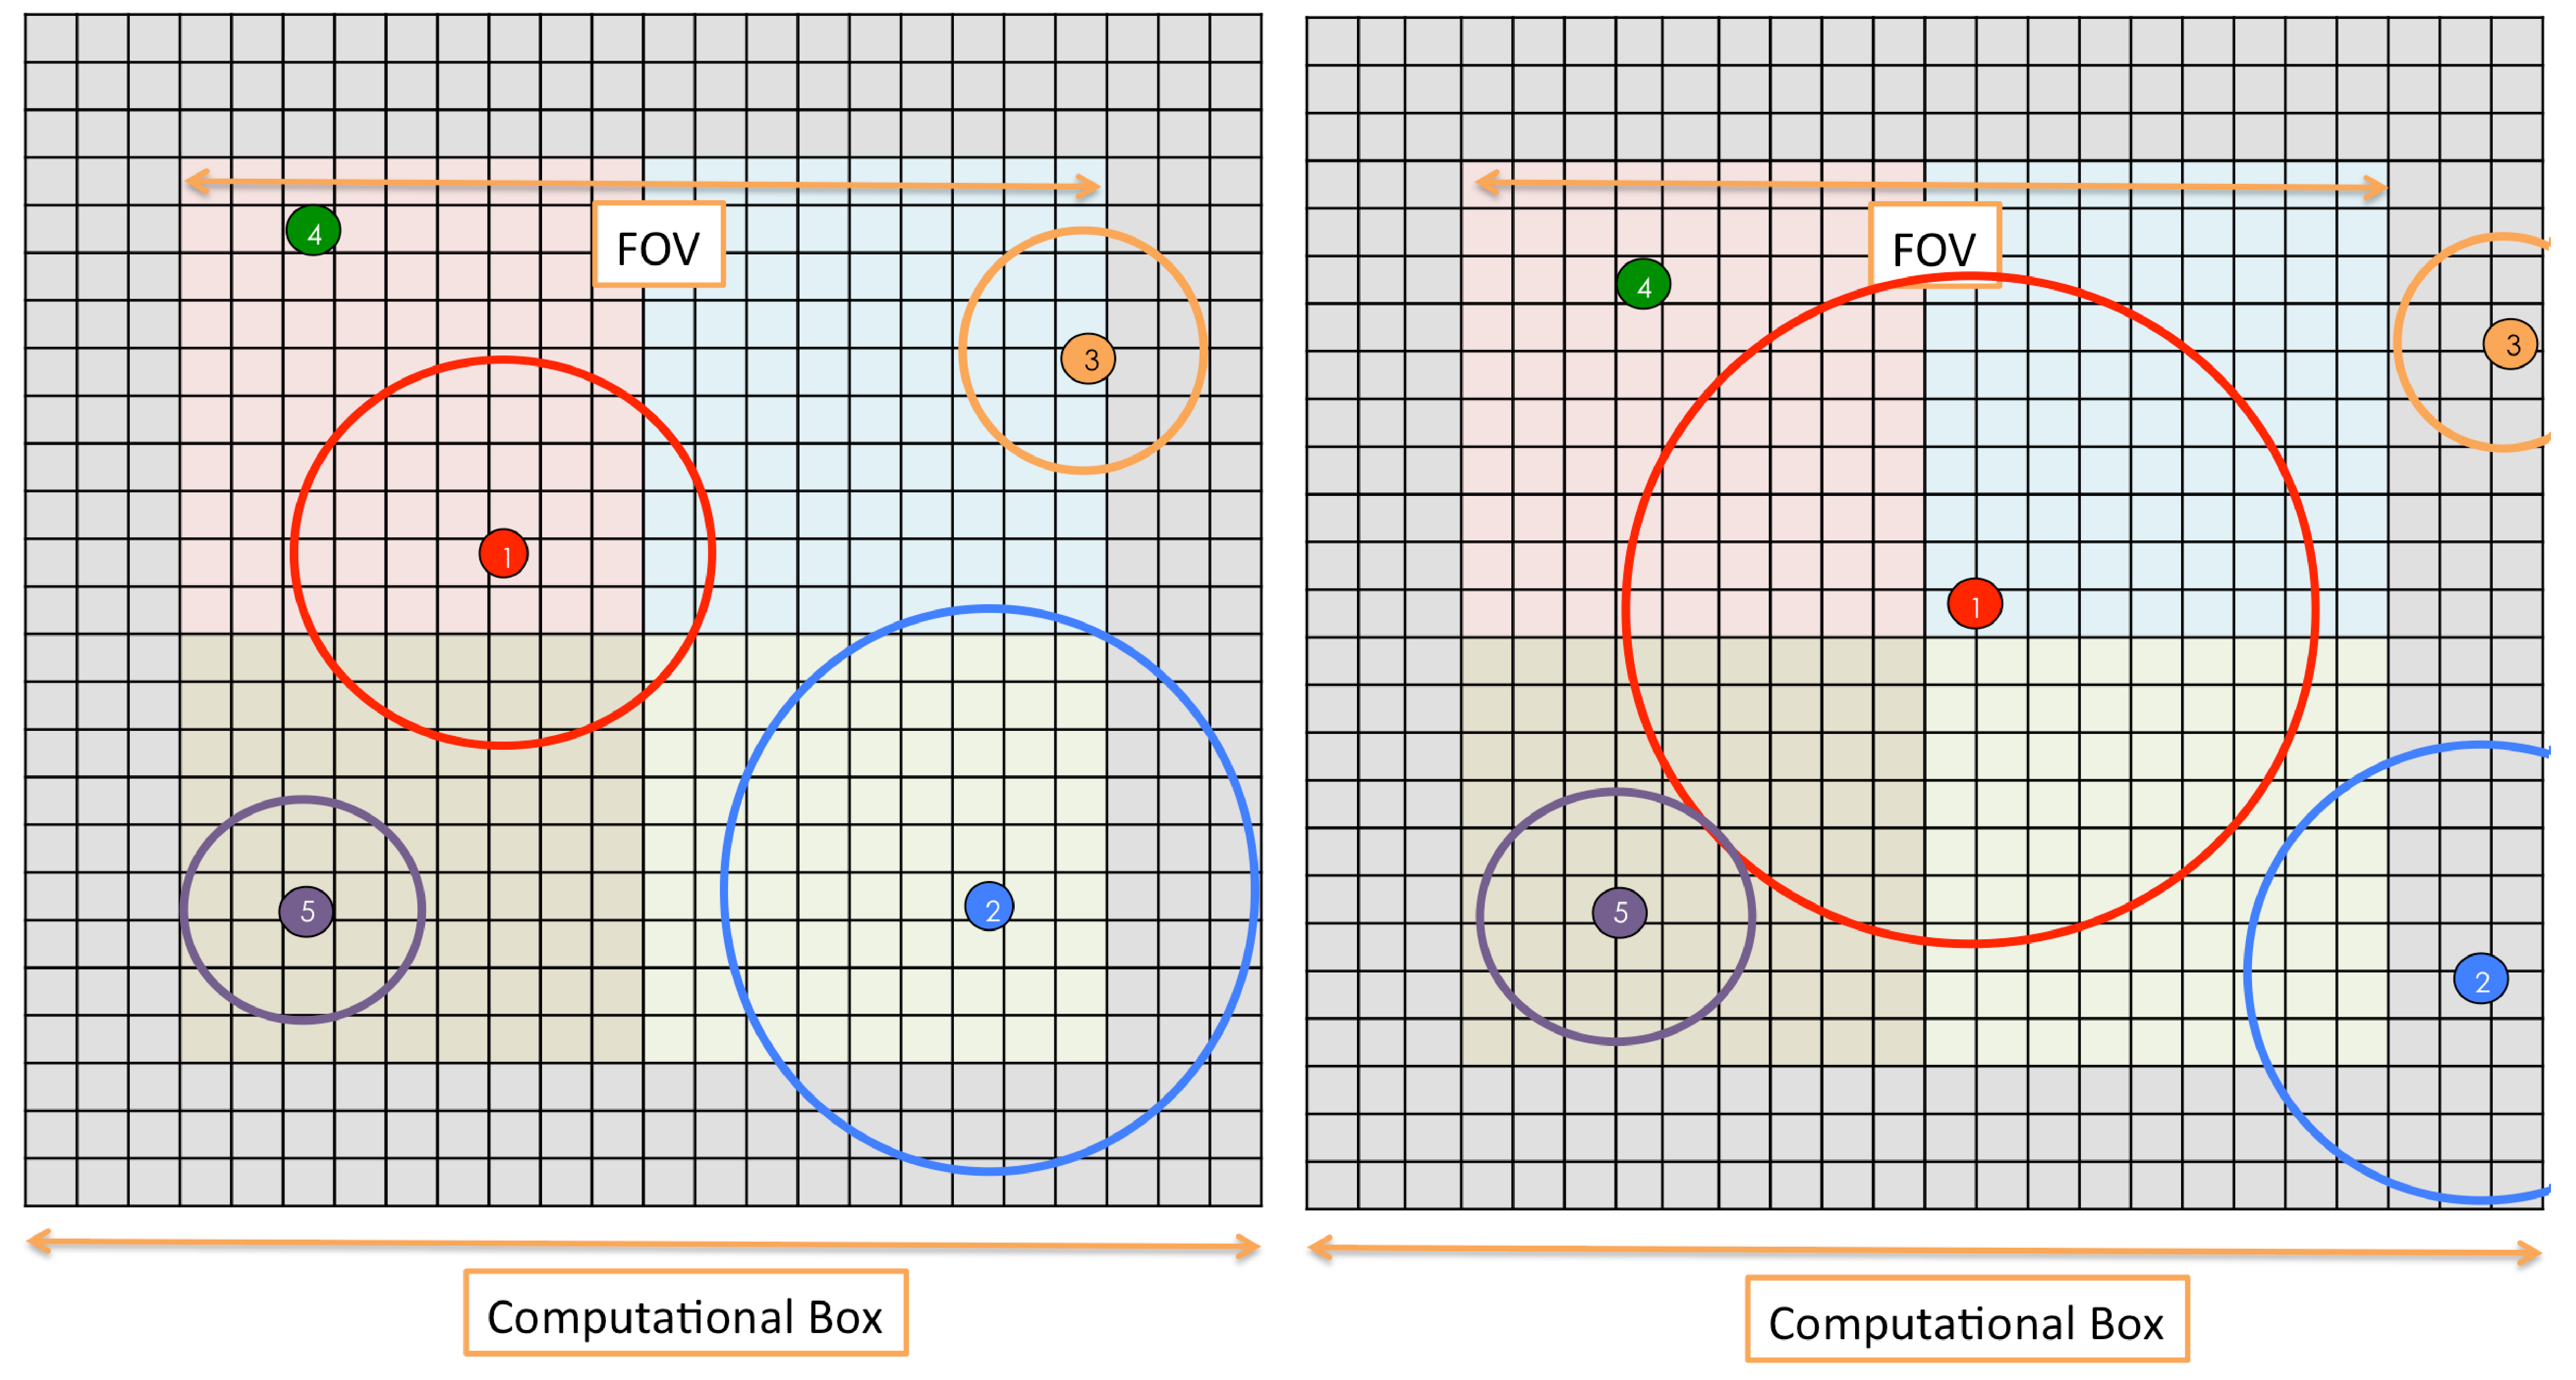
\includegraphics[scale=0.15]{images/fov.eps}
\caption{The scene with five particles from two different points of view. Different tiles are 
represented with different colors. In the first camera position
(left) all particles contributes to the image (lie in the FOV), particles 2 and 3
being classified as C2, particle 4 being C3 and particle 5 being C2. Particle 1, is classified
as C2, since it is completely contained in a {\it Btile} (in this example, it is a tile with a boundary of 3 pixels width). In the right
image the camera moved toward particle 1. All the radii change due to the new point
of view. Classification of particles 4 and 5 does not change, while particle 3 
becomes inactive (completely falling outside the FOV). Particle 2, though 
having coordinates outside the FOV, affects some pixels, hence it is still active.
Particle 1 becomes C1, since its radius exceeds the boundary width, so it exits the Btile. 
}
\label{fig:fov}
\end{figure}



\begin{table}
\caption{Rendering performance results according to different values of the kernel parameters. We set $r_0=8$ and the resolution $N_{pix}=1024$.}
\begin{center}
\begin{tabular}{|l|l|l|l|l|}
\hline
$n_p$ & $t_x$ (pixels) & Kernel & Rendering & Total CUDA \\
& & Occupancy & Time (sec.) & Time (sec.) \\
\hline
256   & 16 & 0.333 & 9.186 & 16.38 \\
\hline
      & 14 & 0.333 & 7.345  & 15.30 \\
\hline
      & 12 & 0.333 & 6.881  & 14.01 \\
\hline
      & 10 & 0.333 & 6.768 & 14.06 \\
\hline
128   & 16 & 0.333 & 9.159 & 17.00 \\
\hline
      & 14 & 0.333 & 7.302  & 15.30 \\
\hline
      & 12 & 0.5 & 5.074  & 12.08 \\
\hline
      & 10 & 0.5 & 5.016 & 12.30 \\ 
\hline
64    & 16 & 0.5 & 6.516 & 14.23 \\
\hline
      & 14 & 0.5 & 5.387 & 12.55 \\
\hline
      & 12 & 0.667 & 4.423 & 11.34 \\
\hline
      & 10 & 0.667 & 4.393 & 11.45 \\ 
\hline
32    & 12 & 0.667 & 4.515 & 12.41 \\
\hline
      & 10 & 0.667 & 4.483 & 12.43 \\ 
\hline
\end{tabular}
\end{center}
\label{tab:tuning}
\end{table}


\bibliographystyle{plain}
\bibliography{master.bib}	

\end{document}
